\section{DAC / ADC}

\subsection{Basics}
Resolution: $N$ Bits \\
$Code = \frac{U_{IN}}{U_{FS}} \cdot 2^N$ / $U_{IN} = Code \cdot \frac{U_{FS}}{2^N}$ / $U_{FS} = U_{ref}$ (Single ended) / $U_{FS} = 2 \cdot U_{ref}$ (Differential)\\
$U_{LSB} = \frac{U_{FS}}{2^N}$

\subsection{Noise}
Signal to Noise: $SNR_{db} = 10 \cdot \log_{10}(\frac{P_{signal}}{P_{noise}}) = 20 \cdot \log_{10}(\frac{U_{signal}}{U_{noise}})$\\
Noise due Quantization: $U_{N,RMS} = \frac{U_{LSB}}{\sqrt{12}}$\\
Signal to Noise due Quantization assuming full scale sine input: $SNR_{db} = 1.76 + N \cdot 6.02$\\
Distortion (Based on Fourier series): In: $A_1 \sin(\omega t)$ Out: $A_1 \sin(\omega t) + A_2 \sin(2 \omega t) + \hdots$ $\rightarrow$ $\text{THD} = \sqrt{\frac{A_1^2}{A_2^2 + A_3^2 + \hdots}}$\\
Singnal-to-Noise and Distortion: $SINAD_{db} = 10 \cdot \log_{10}\left(\frac{A_1^2}{P_{noise} + A_2^2 + A_3^2 + \hdots}\right)$\\
Effective Number of Bits: $ENOB = \frac{SINAD_{db} - 1.76}{6.02}$\\
Spurious Free Synamic Range:\\
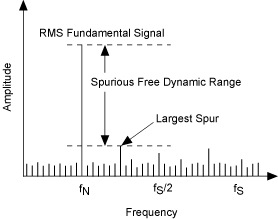
\includegraphics[
		width=0.3\textwidth,
		keepaspectratio,
		angle=0
		]{images/DacAdc/sfdr}

\subsection{Non Lineraries}

\begin{tabular}{m{5cm} m{5cm} m{5cm}}
 	Offset error & Gain Error & \\ 
	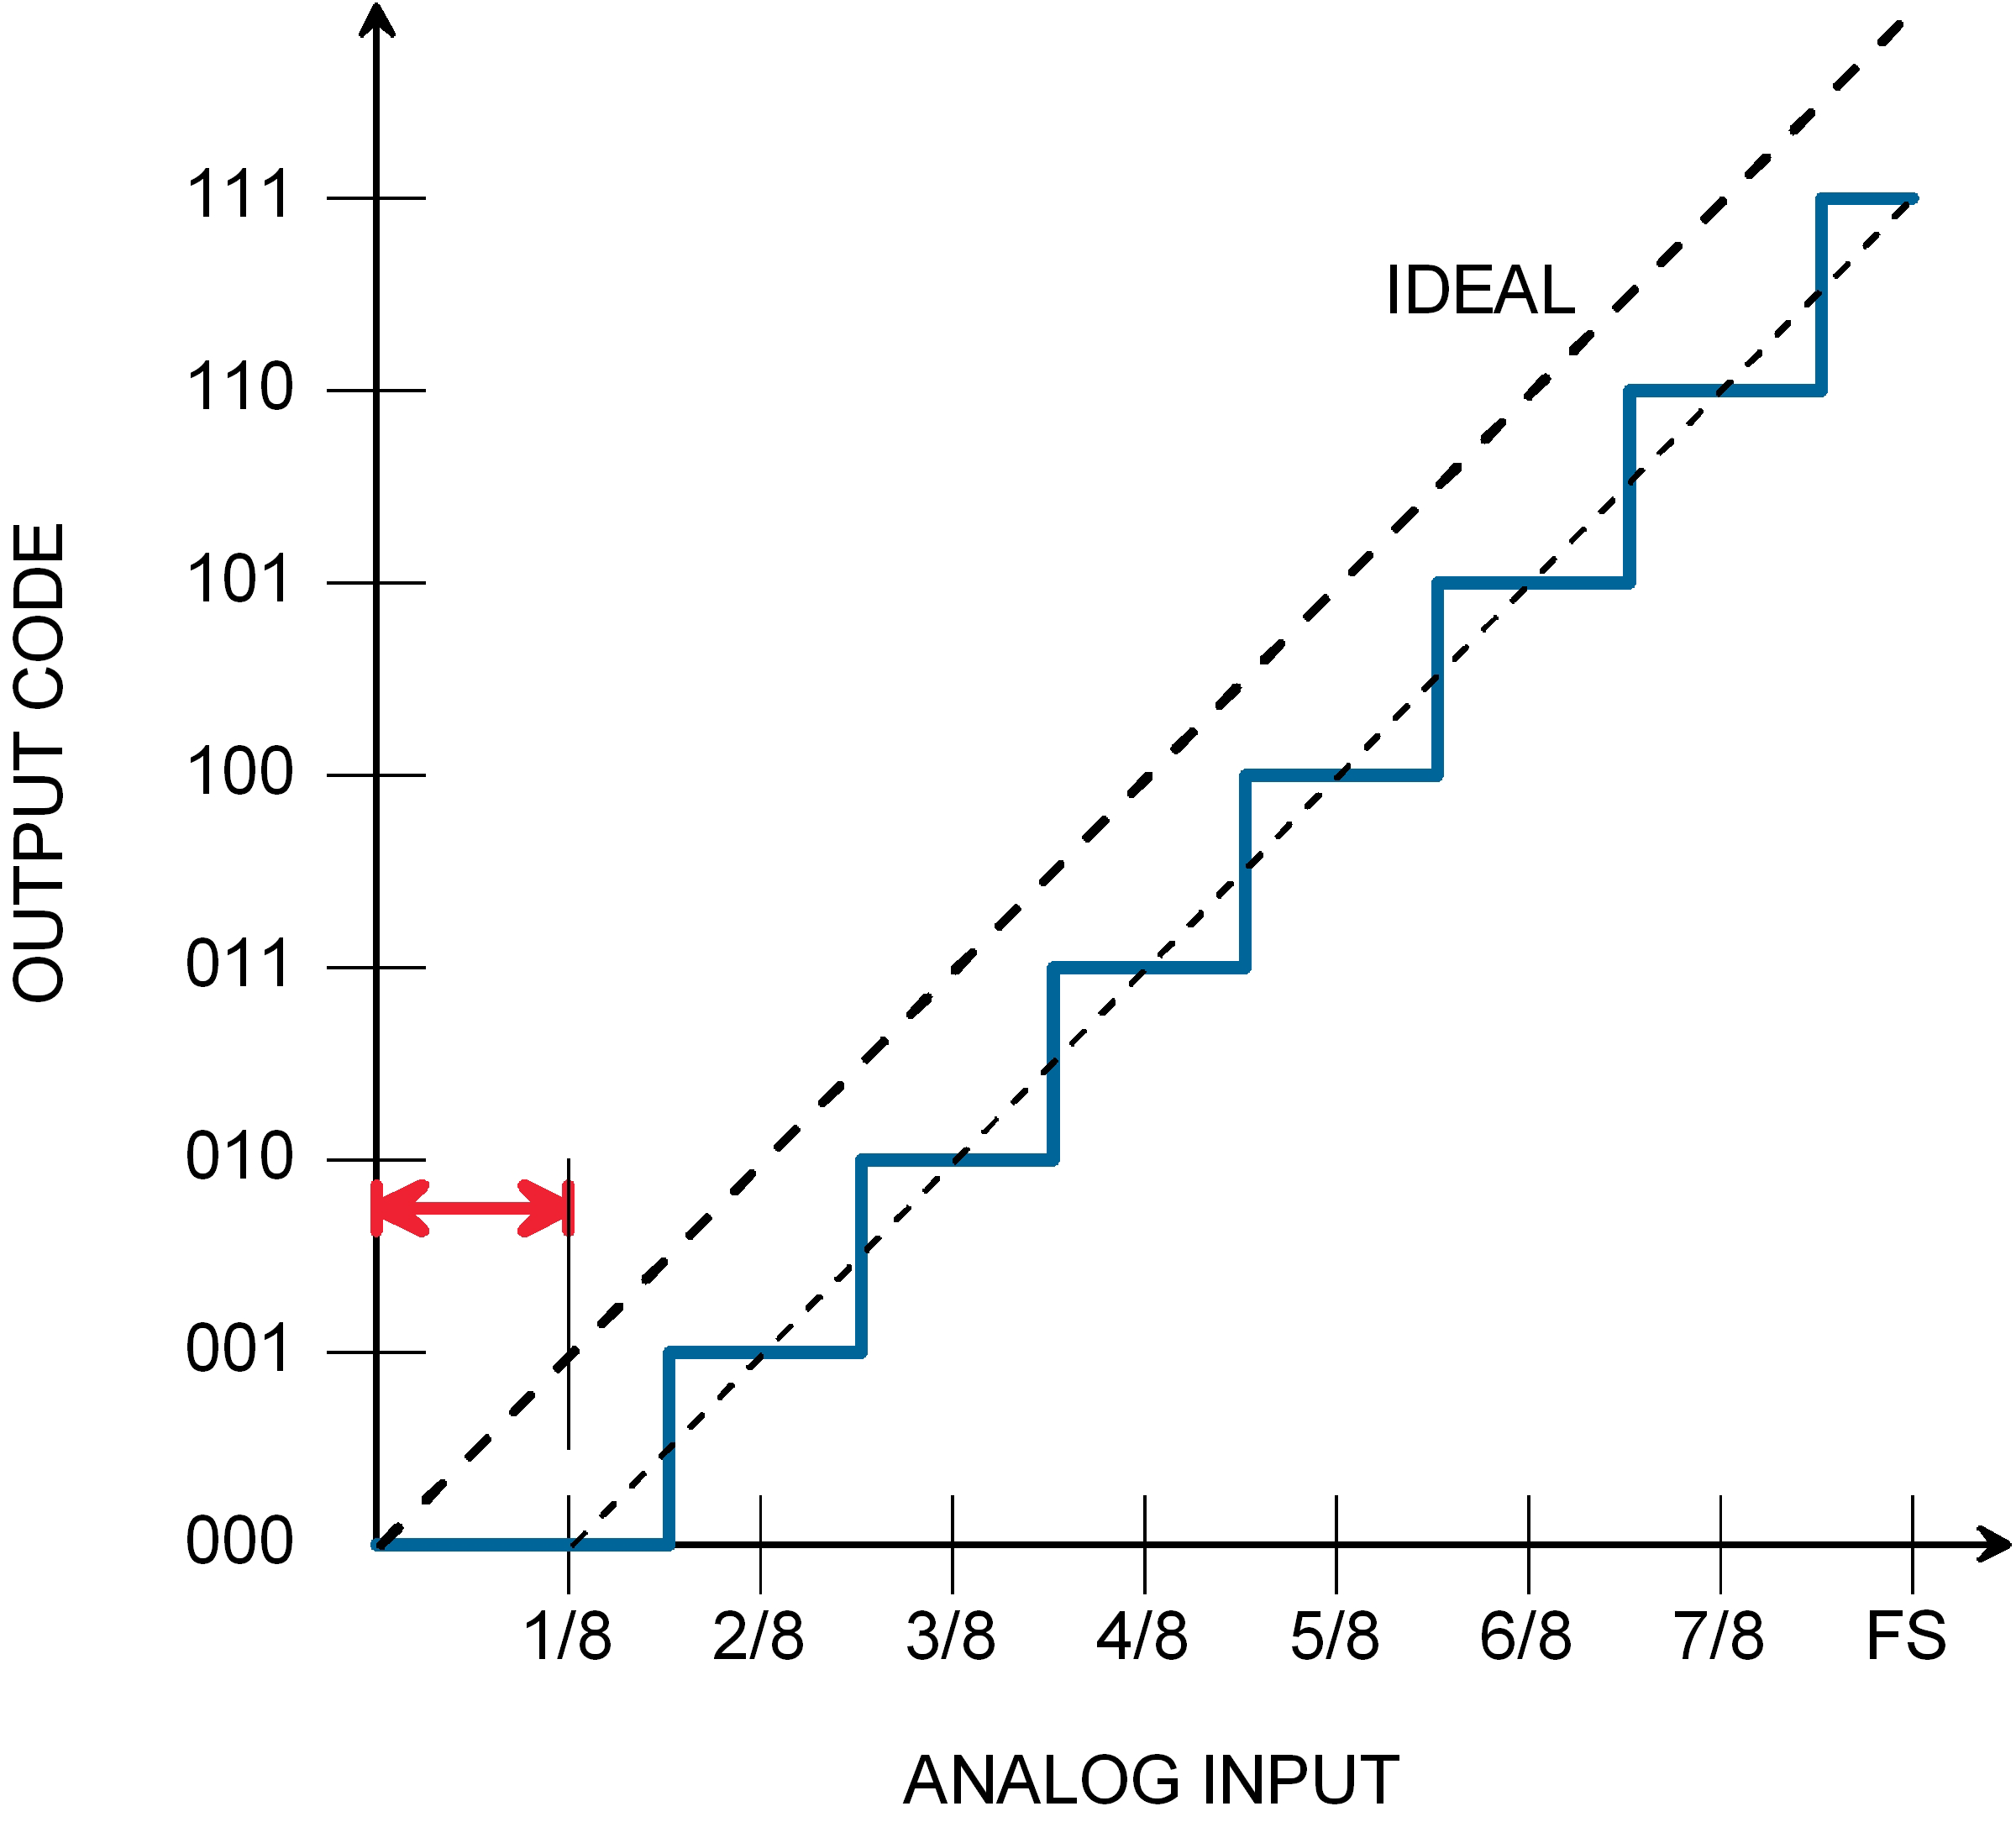
\includegraphics[
		width=0.25\textwidth,
		keepaspectratio,
		angle=0
		]{images/DacAdc/offset} & 
	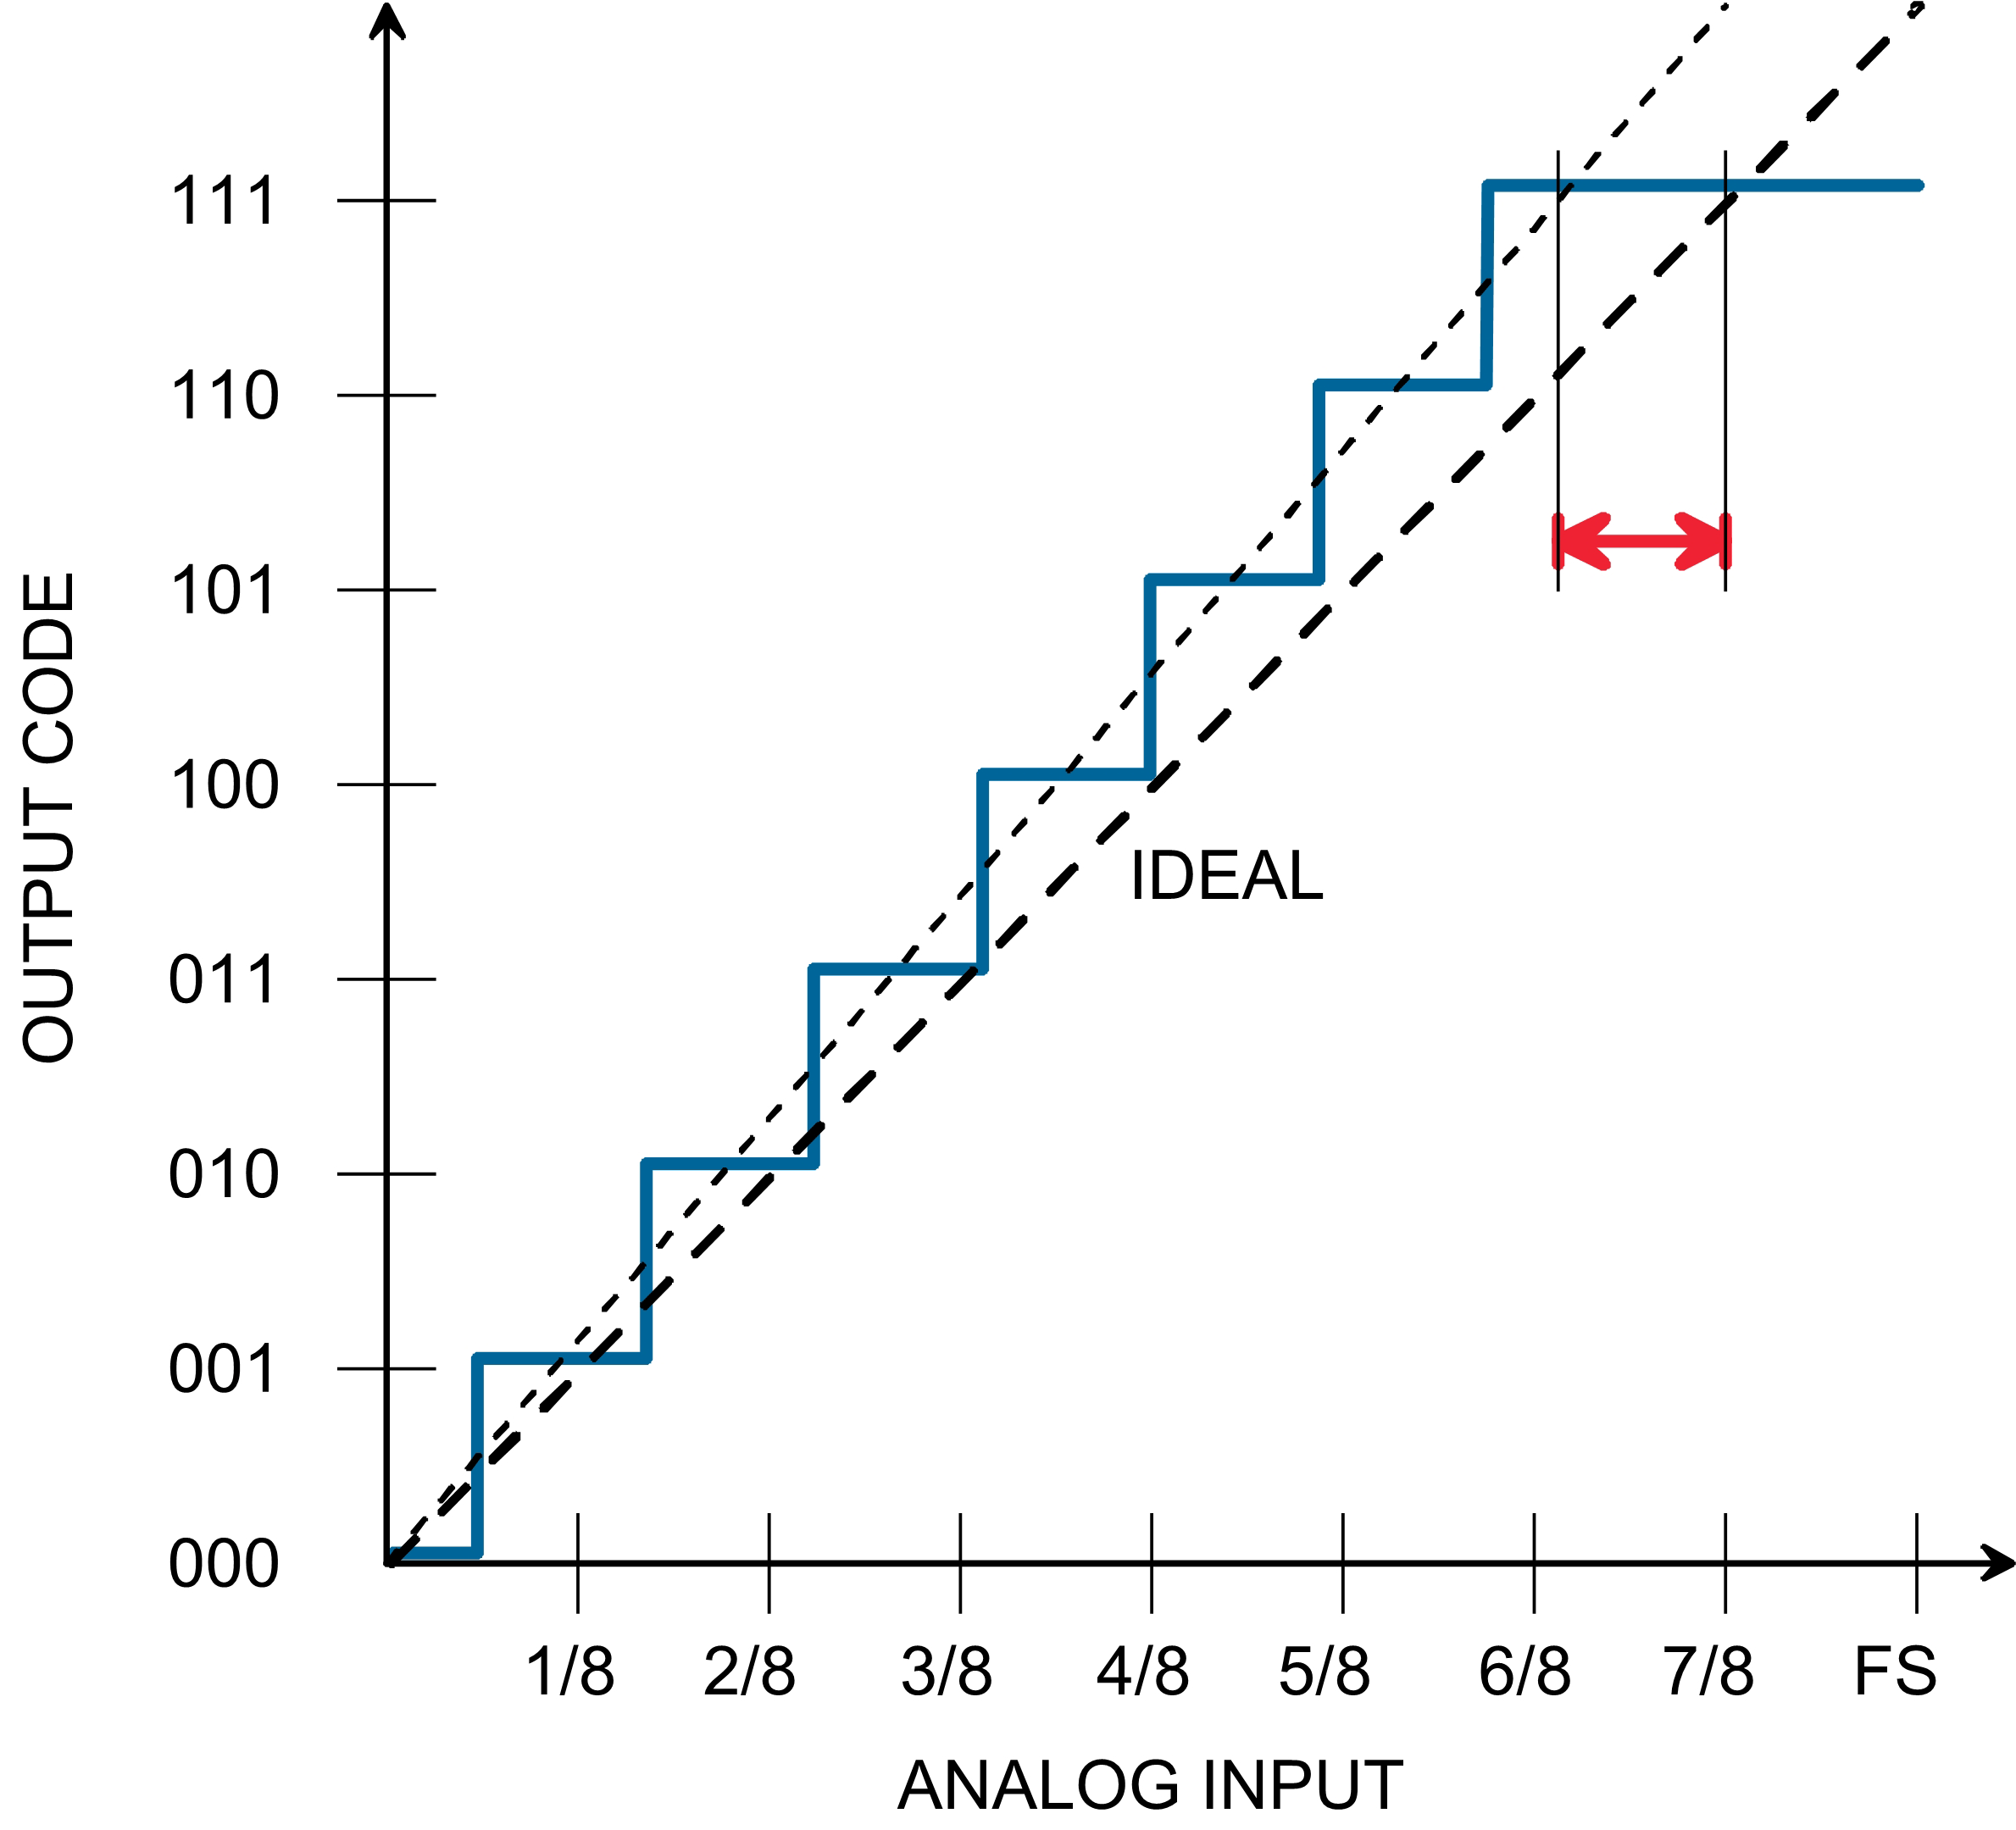
\includegraphics[
		width=0.25\textwidth,
		keepaspectratio,
		angle=0
		]{images/DacAdc/gain} & \\ 
		
	INL / DNL & Missing Codes & \\ 
	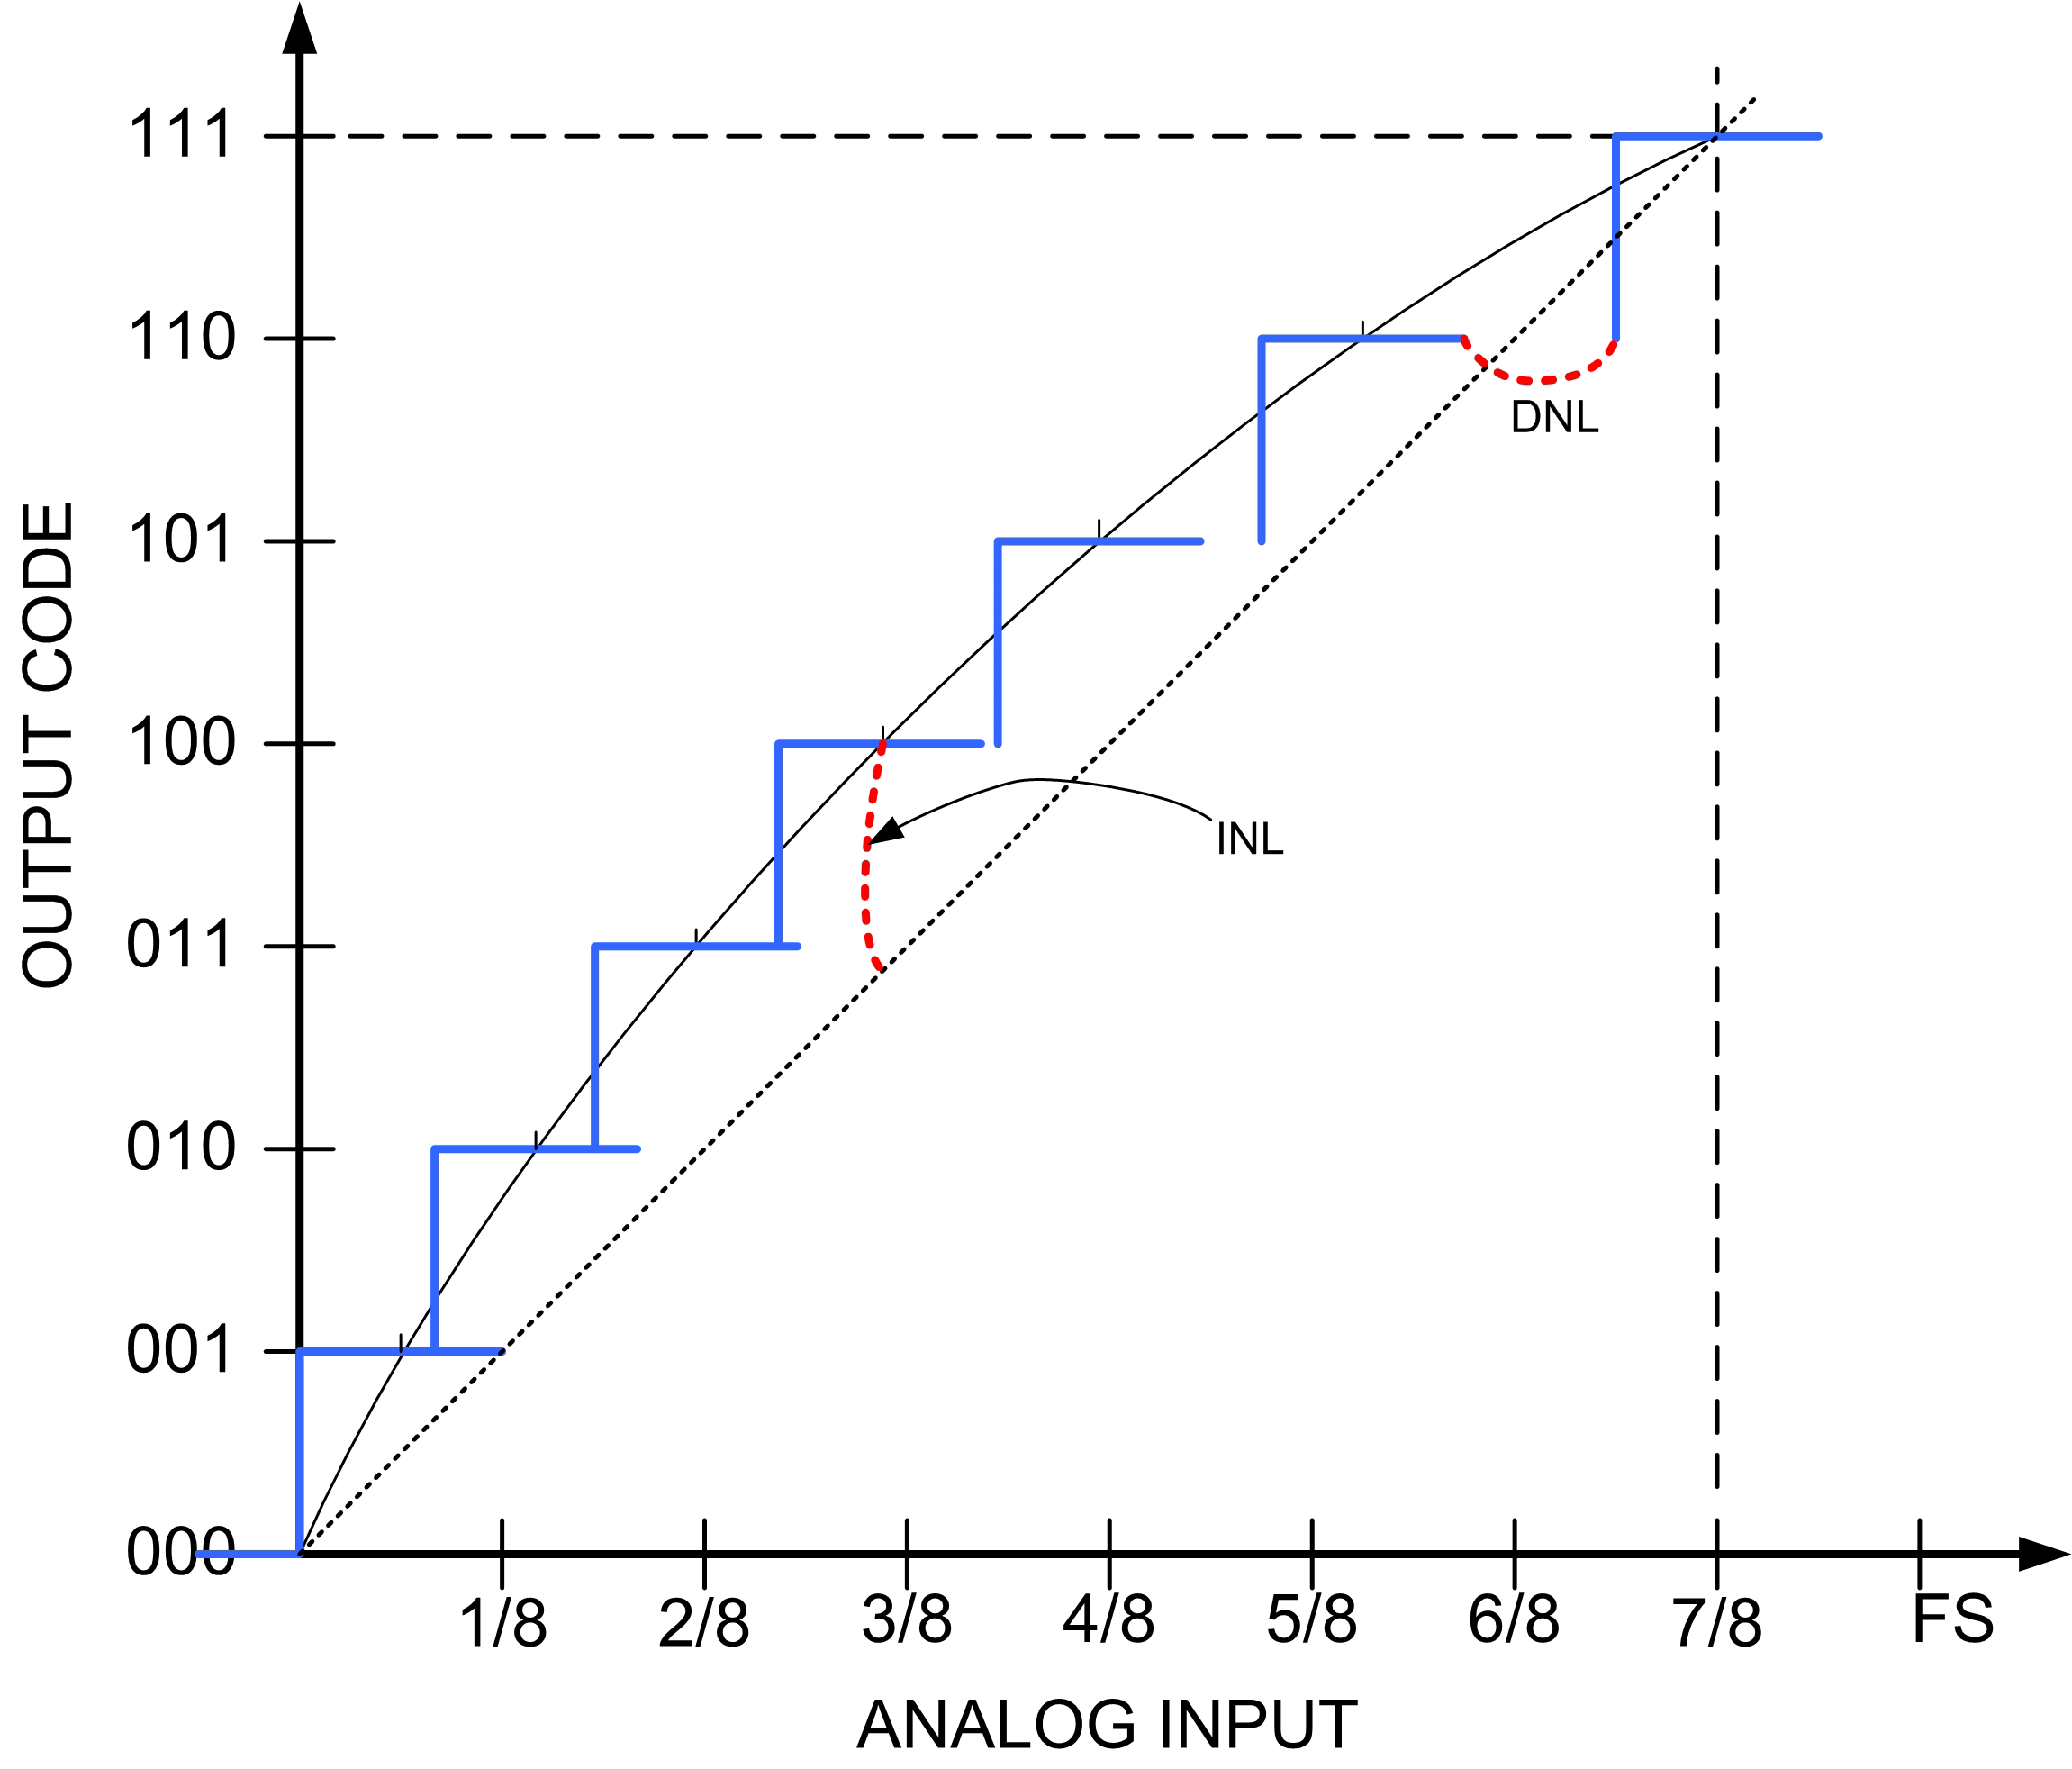
\includegraphics[
		width=0.25\textwidth,
		keepaspectratio,
		angle=0
		]{images/DacAdc/inl_dnl} & 
	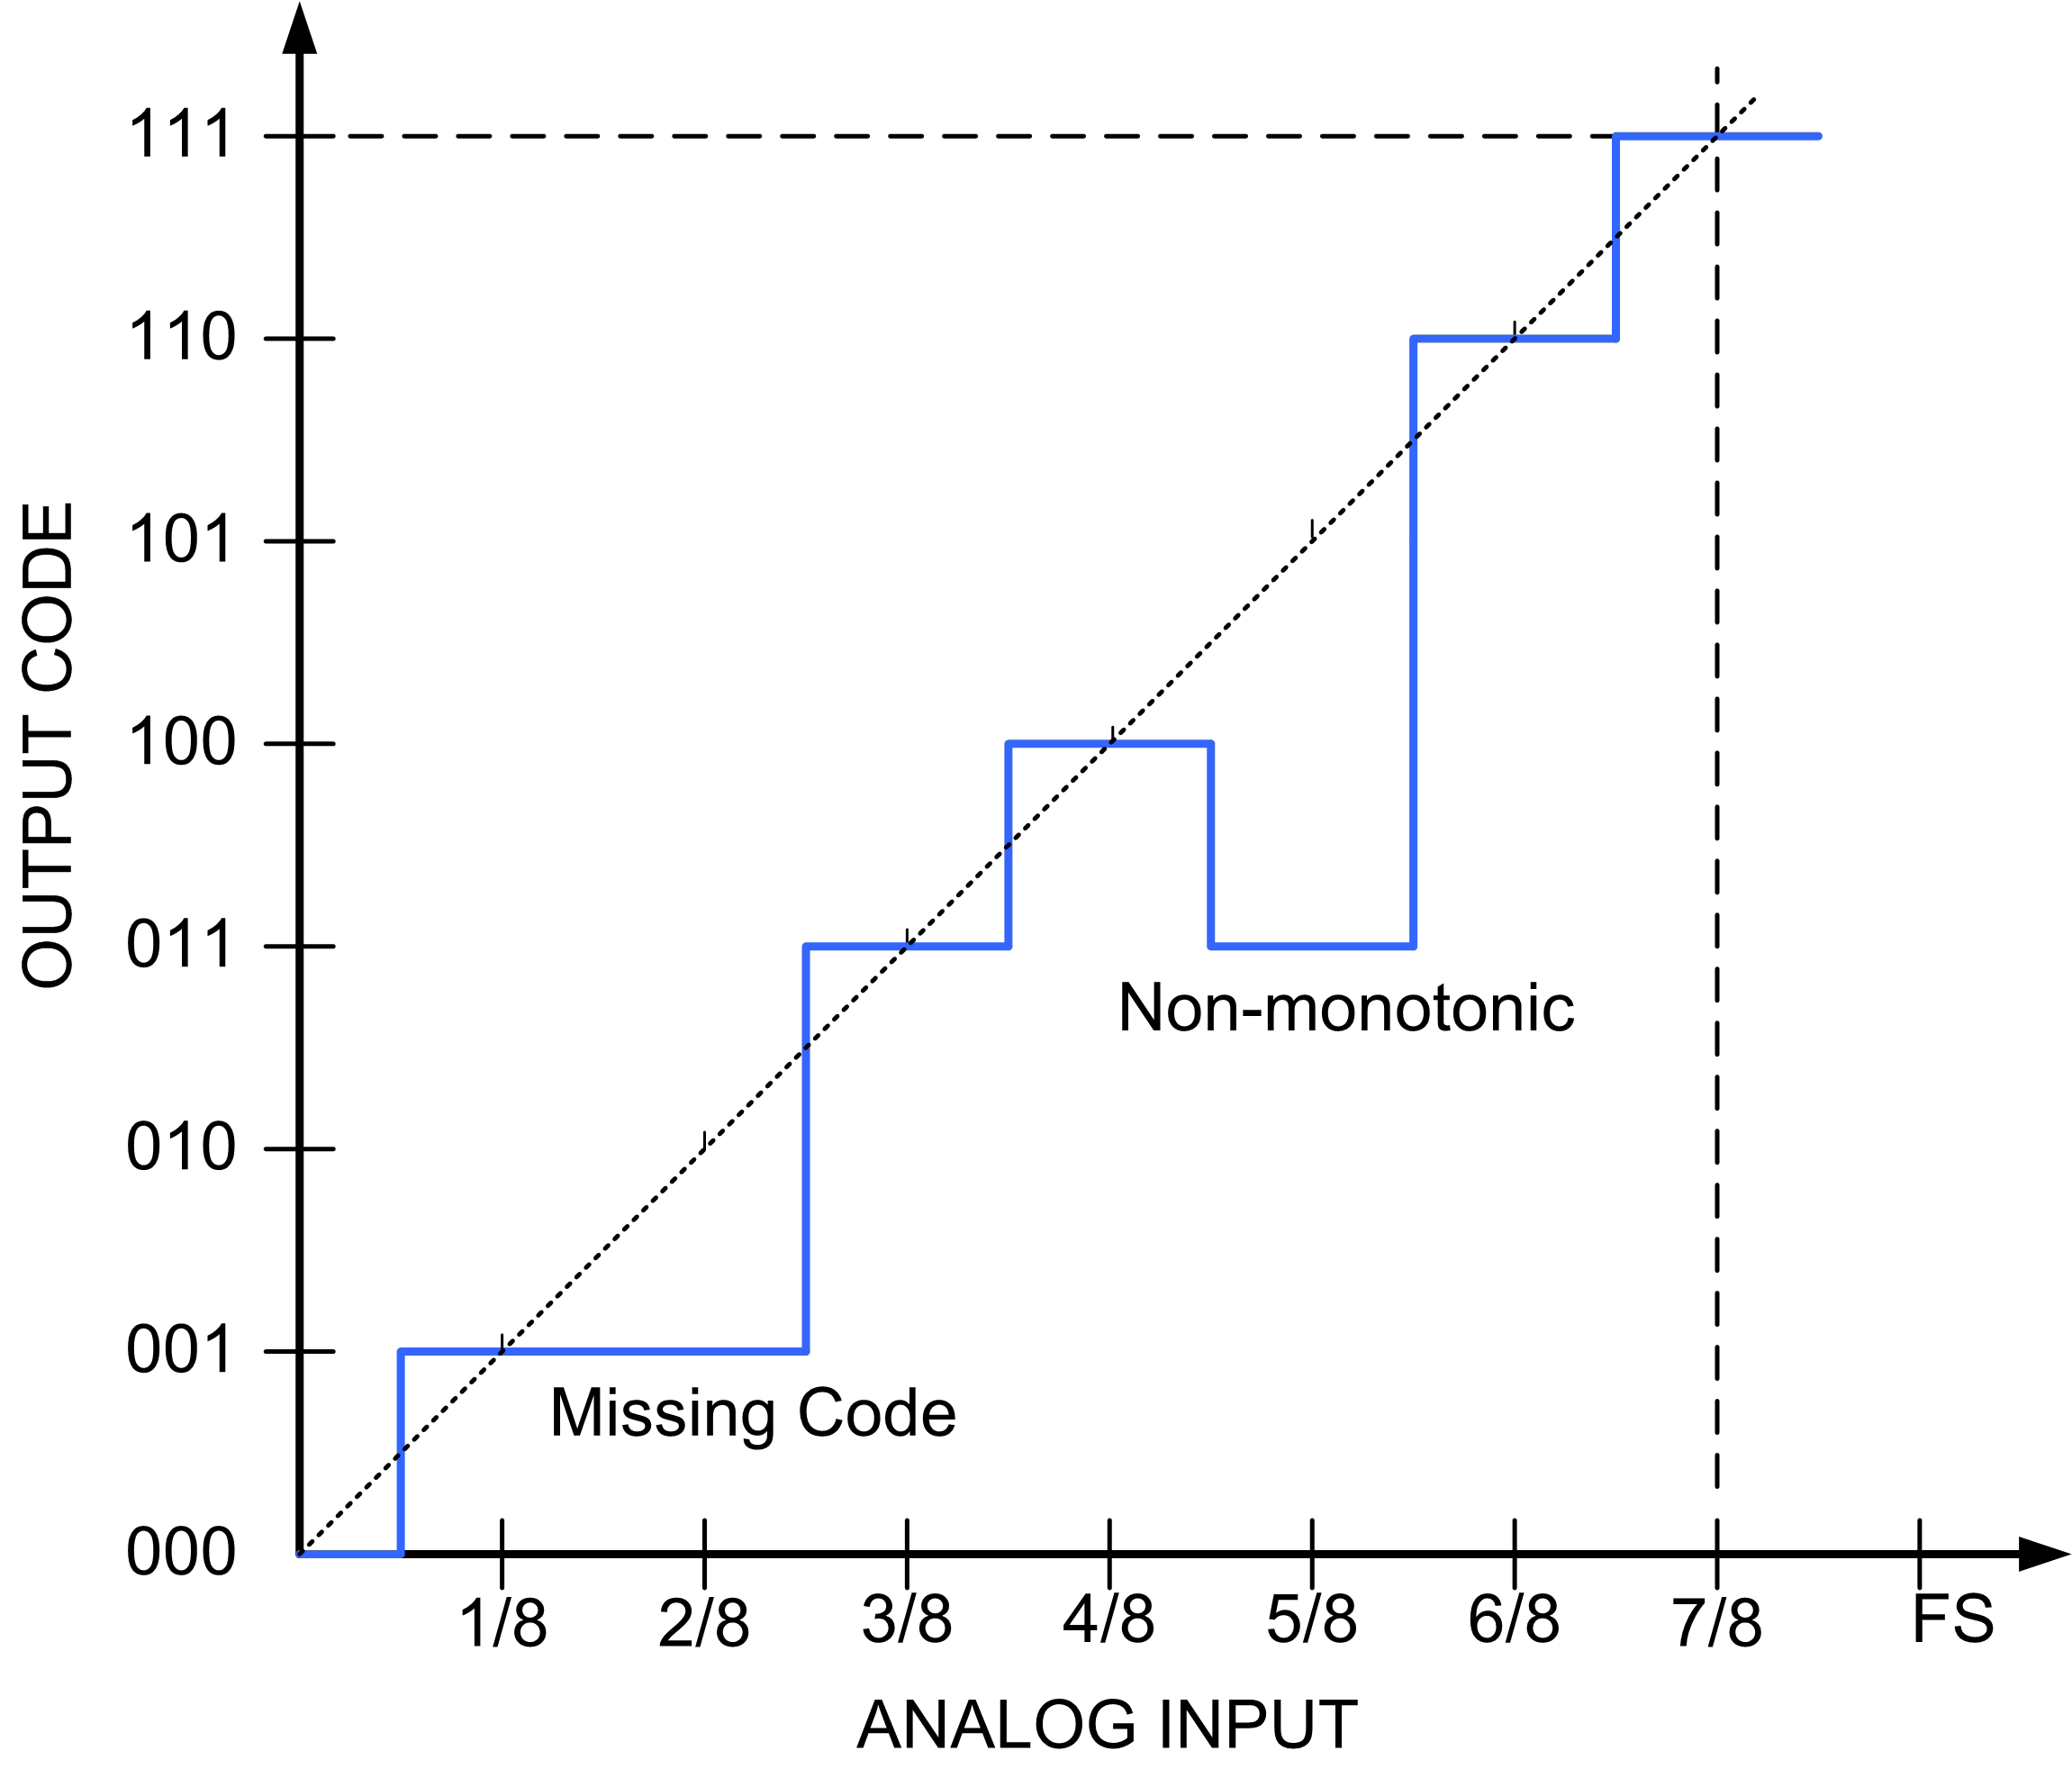
\includegraphics[
		width=0.25\textwidth,
		keepaspectratio,
		angle=0
		]{images/DacAdc/missing_codes} & 
		\begin{minipage}{0.4\textwidth}
		\begin{itemize}
			\item DNL $< -1$ $\rightarrow$ Non-monotonic
			\item DNL $> +1$ $\rightarrow$ Missing Code
		\end{itemize}
		\end{minipage}\\ 

\end{tabular}

\subsection{DAC}
Unitary: Monotonicity guaranteed but needs $2^N$ elements!

\begin{tabular}{m{8cm} m{6cm}}
 	Kelvin Divider & Segmented Chains \\ 
	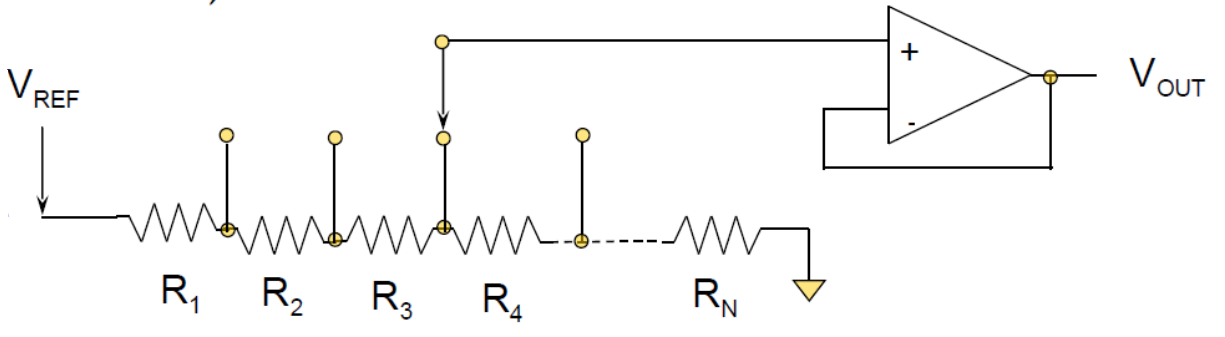
\includegraphics[
		width=8cm,
		keepaspectratio,
		angle=0
		]{images/DacAdc/kelvin_divider} & 
	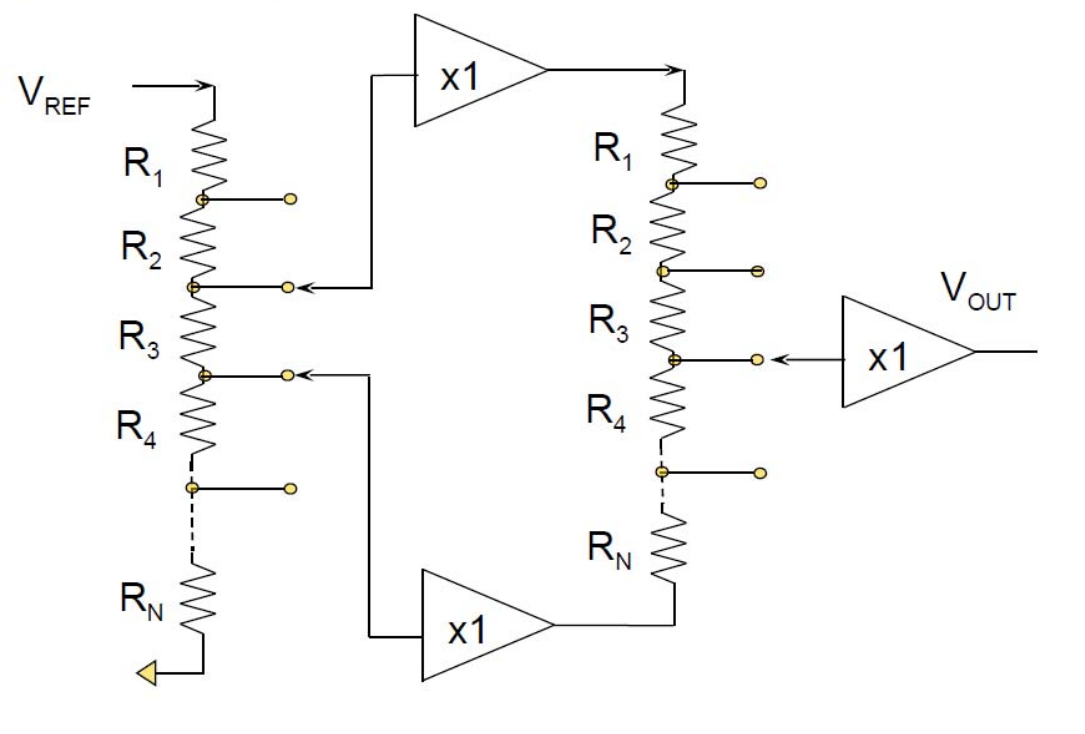
\includegraphics[
		width=6cm,
		keepaspectratio,
		angle=0
		]{images/DacAdc/segmented_chain} \\ 
\end{tabular}

Binary: No monotonicity guaranteed but needs just $N$ elements!

\begin{tabular}{m{8cm} m{8cm}}
 	Binary weighted & R-2R structure \\ 
	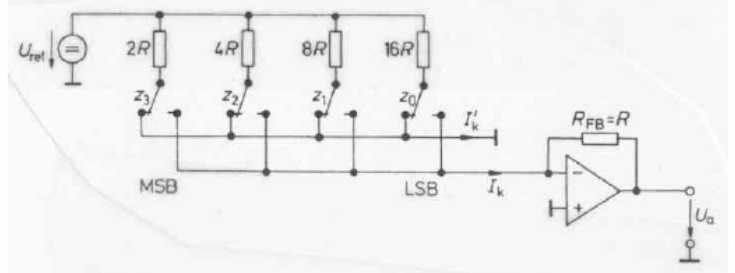
\includegraphics[
		width=8cm,
		keepaspectratio,
		angle=0
		]{images/DacAdc/binary_weighted} & 
	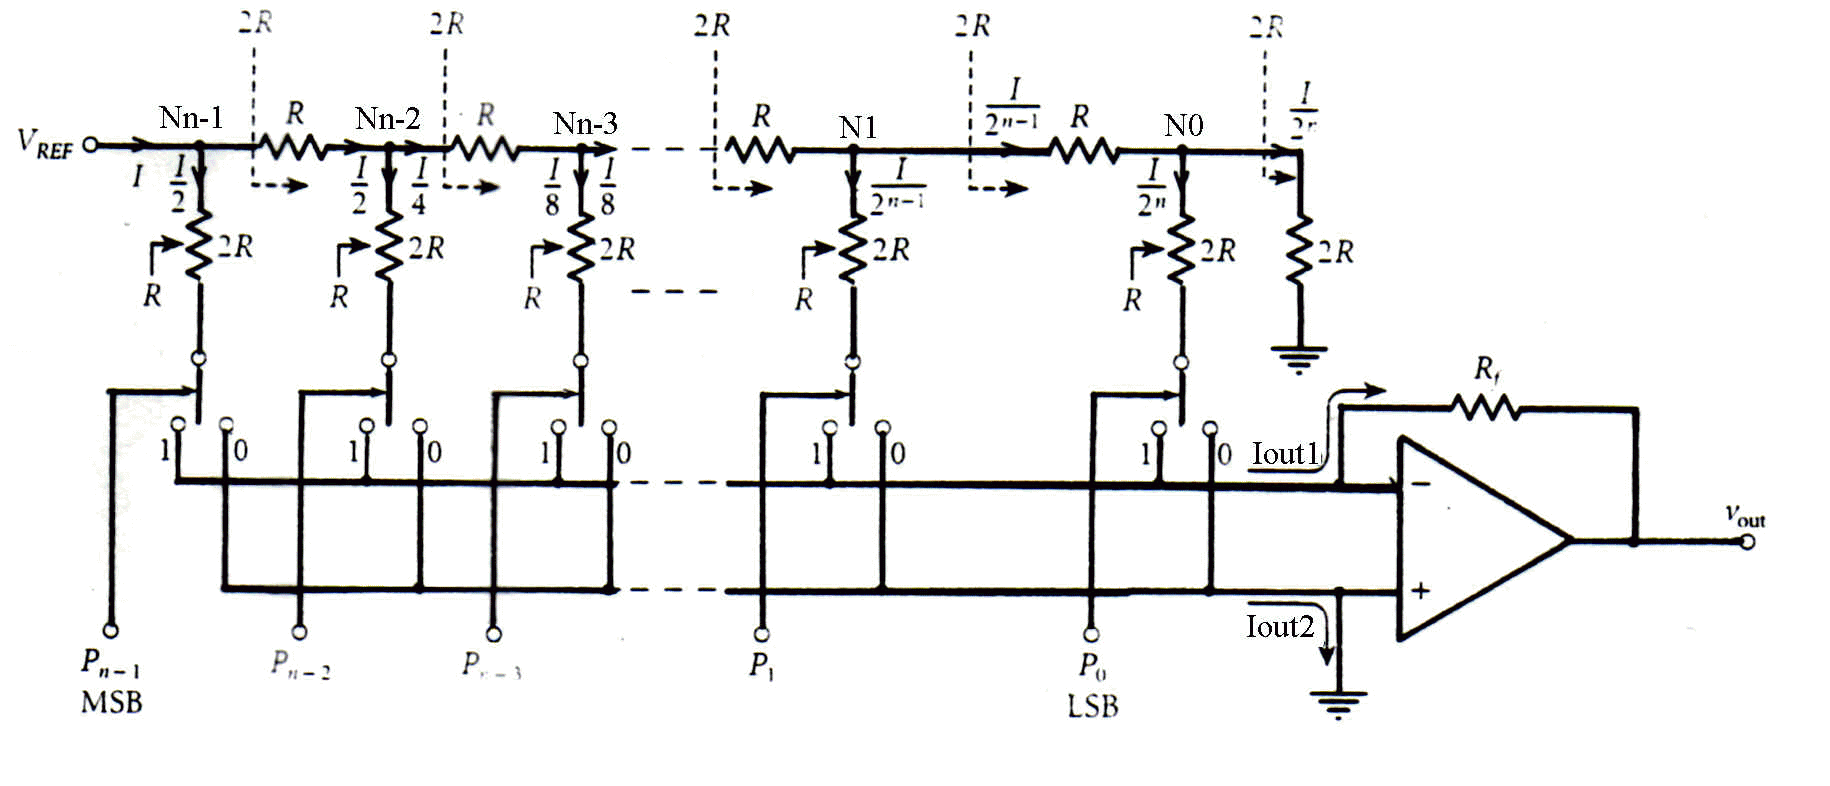
\includegraphics[
		width=8cm,
		keepaspectratio,
		angle=0
		]{images/DacAdc/r_2r} \\ 
\end{tabular}